\documentclass[12pt]{article}
\usepackage{graphicx}
\usepackage{amsmath,amssymb,amsthm}
\usepackage{geometry}
\geometry{margin=1in}
\usepackage{hyperref}
\usepackage{tikz}
\usetikzlibrary{positioning,arrows.meta}
\usepackage{booktabs}
\usepackage{authblk}

\newtheorem{theorem}{Theorem}
\newtheorem{proposition}[theorem]{Proposition}
\newtheorem{lemma}[theorem]{Lemma}
\theoremstyle{definition}
\newtheorem{definition}[theorem]{Definition}
\newtheorem{remark}[theorem]{Remark}

\title{Geometric Unification of Flavor:\\ Masses, Mixing, and CP from the Golden Ratio Lattice}
\author[1]{Marvin L. Gentry}
\affil[1]{Independent Researcher, \texttt{drmlgentry@protonmail.com} \\ ORCID: 0009-0006-4550-2663}
\date{\today}

\begin{document}
\maketitle

\begin{abstract}
We present a unified geometric framework for Standard Model flavor: fermion masses, mixing matrices, and CP-violating phases are consistent with arising from the structure of a single arithmetic lattice embedded in a symmetric space. The key observation is that the observed fermion masses cluster near the discrete set
\[
m = m_e \cdot \phi^{\,q/4}, \qquad q\in\mathbb{Z},
\]
where $\phi = (1+\sqrt5)/2$ is the golden ratio and $m_e$ the electron mass. This lattice is precisely the image of the logarithmic unit lattice of $\mathbb{Q}(\sqrt5)$ under the exponential map of the symmetric space $\mathrm{SL}(2,\mathbb{R})/\mathrm{SO}(2)$ (the hyperbolic plane), with covolume $\log\phi$. The quarter‑integer spacing arises from the metric normalization of the maximal flat.

We demonstrate that the same geometric construction extends to mixing and CP violation via the Iwasawa decomposition $\mathrm{PSL}(2,\mathbb{C}) = KAN$ (Figure~\ref{fig:kan}): the $K$‑ and $N$‑factors encode the CKM and PMNS mixing matrices (companion papers), while the $A$‑factor (twist angles) gives CP phases that are holonomies of flat $\mathrm{U}(1)$ connections classified by the torsion $H_1(M)=\mathbb{Z}/5$ of the underlying hyperbolic 3‑manifolds. The entire flavor sector is thus encoded in the discrete geometry of a single arithmetic lattice and its associated symmetric space.

All results are presented under a strict methodological contract: fixed conventions, bounded scans, explicit falsifiability criteria. Residuals are stable and small; null tests confirm non‑random clustering. The framework provides a geometric origin for the golden ratio in particle physics and unifies masses, mixing, and CP in a single arithmetic‑geometric structure.
\end{abstract}

\section{Introduction}
\label{sec:intro}

The flavor parameters of the Standard Model—fermion masses, mixing angles, and CP phases—are among the most precisely measured quantities in particle physics, yet their origin remains unexplained. The observed mass hierarchy spans more than twelve orders of magnitude, and the mixing matrices exhibit a characteristic pattern often described as “Cabibbo suppression” and “weak mixing.” Many theoretical approaches invoke discrete flavor symmetries, extra dimensions, or string‑inspired constructions, but they typically introduce free parameters and lack a unifying geometric principle.

In this work we propose that the entire flavor structure is consistent with being encoded in a single arithmetic lattice embedded in a symmetric space. The lattice is the logarithmic unit lattice of the quadratic field $\mathbb{Q}(\sqrt5)$, which appears naturally in the geometry of the symmetric space $\mathrm{SL}(2,\mathbb{R})/\mathrm{SO}(2)$ (the hyperbolic plane). Its covolume is the regulator $\log\phi$, where $\phi = (1+\sqrt5)/2$ is the golden ratio. Under the exponential map of the symmetric space, this lattice gives the discrete set
\[
m = m_e \cdot \phi^{\,q/4},\qquad q\in\mathbb{Z},
\]
where the quarter‑integer spacing emerges from the metric normalization of the maximal flat.

Remarkably, this set coincides with the observed fermion masses: the electron defines $q=0$, the muon and tau cluster near $q=44$ and $q=68$, the light quarks near $q=12,18,43$, the heavy quarks near $q=65,75,106$, and the $W$, $Z$, and Higgs bosons near $q=99,101,103$ (Table~\ref{tab:masses}). The residuals are small, typically a few percent in mass ratio, and the pattern is stable under perturbations of input values.

Beyond masses, the same geometric framework accommodates mixing and CP violation. The Iwasawa decomposition $\mathrm{PSL}(2,\mathbb{C}) = KAN$ of the holonomy group of a compact hyperbolic 3‑manifold provides a natural split: the $K$‑factor (maximal compact) gives the CKM quark mixing matrix, the $N$‑factor (unipotent) gives the PMNS lepton mixing matrix, and the $A$‑factor (diagonal) gives CP phases as flat $\mathrm{U}(1)$ holonomies. The underlying manifolds—$m006$ for quarks and $m003$ for leptons—both have first homology $H_1 = \mathbb{Z}/5$, which quantizes the CP phase to a fifth root of unity, matching the observed Jarlskog invariant. The connection between the mass lattice and the mixing sector (Figure~\ref{fig:framework}) is indirect but unified: both stem from the same arithmetic hyperbolic geometry.

We identify the precise arithmetic mechanism linking the two sectors. The torsion $H_1(M)=\mathbb{Z}/5$ classifies flat $\mathrm{U}(1)$ connections on $M$ via characters $\chi: \mathbb{Z}/5 \to \mathrm{U}(1)$, giving holonomies $e^{2\pi i k/5}$ --- fifth roots of unity. These generate the cyclotomic field $\mathbb{Q}(\zeta_5)$, whose maximal real subfield is $\mathbb{Q}(\zeta_5 + \zeta_5^{-1}) = \mathbb{Q}(\sqrt{5})$, with fundamental unit $\phi = (1+\sqrt{5})/2$. The regulator of $\mathbb{Q}(\sqrt{5})$ is $\log\phi$, which is precisely the lattice spacing of the mass formula. In particular, $2\cos(2\pi/5) = \phi - 1 = 1/\phi$, so the CP phase $e^{2\pi i/5}$ and the golden ratio $\phi$ are two facets of the same $\mathbb{Z}/5$ structure. The entire flavor sector is thus tied to the single arithmetic datum $H_1(M) = \mathbb{Z}/5$.

This paper is structured as a methodological and empirical synthesis. Section~\ref{sec:geom} recalls the symmetric‑space construction and derives the mass lattice. Section~\ref{sec:methods} describes the encoding, anchoring, scan protocol, and null tests in detail. Section~\ref{sec:mass_results} presents the mass clustering results. Section~\ref{sec:mixing_cp} outlines the extension to mixing and CP violation, referencing companion papers. Section~\ref{sec:spectral} discusses the spectral properties of the underlying manifolds. Section~\ref{sec:discussion} discusses falsifiability, interpretive limits, and future directions. Section~\ref{sec:conclusion} concludes.

\section{Geometric foundation: the golden ratio lattice}
\label{sec:geom}

The key geometric input comes from the theory of symmetric spaces and arithmetic groups. The space of positive definite quadratic forms modulo overall scale is the symmetric space
\[
\mathcal{M}_n = \mathrm{SL}(n,\mathbb{R})/\mathrm{SO}(n)
\]
(see \cite{Gentry:ShapeSpace} for a detailed exposition). Its tangent space at the identity is the space of traceless symmetric matrices. A maximal flat is obtained by exponentiating the Cartan subalgebra of diagonal matrices with zero trace, which is isometric to $\mathbb{R}^{n-1}$ with the Euclidean metric $\langle X,Y\rangle = \operatorname{tr}(XY)$.

For $n=2$, $\mathcal{M}_2 \cong \mathrm{SL}(2,\mathbb{R})/\mathrm{SO}(2)$ is the hyperbolic plane. Its maximal flats are geodesics. The real quadratic field $K = \mathbb{Q}(\sqrt5)$ has unit group $\mathcal{O}_K^\times \cong \{\pm1\}\times\mathbb{Z}$. The logarithmic embedding maps units to vectors in $\mathbb{R}^2$:
\[
\varepsilon \longmapsto (\log|\sigma_1(\varepsilon)|,\ \log|\sigma_2(\varepsilon)|),
\]
where $\sigma_{1,2}$ are the two real embeddings. Because $N_{K/\mathbb{Q}}(\varepsilon)= \sigma_1(\varepsilon)\sigma_2(\varepsilon) = \pm1$, the image lies in the line $x_1+x_2=0$, which can be identified with the Lie algebra $\mathfrak{a} = \operatorname{Diag}_0(2,\mathbb{R}) = \{\operatorname{diag}(t,-t) : t\in\mathbb{R}\}$.

The fundamental unit $\varepsilon_0 = \phi = \frac{1+\sqrt5}{2}$ gives $\Lambda(\phi)= (\log\phi, -\log\phi)$. Its covolume in $\mathfrak{a}$ (the regulator) is $R_K = \log\phi$.

Under the exponential map $\exp:\mathfrak{a}\to\mathcal{M}_2$, the lattice $\mathbb{Z}\cdot\Lambda(\phi)$ maps to the discrete set
\[
\left\{ \exp\!\bigl(t\operatorname{diag}(1,-1)\bigr) : t = k\log\phi \right\}
= \left\{ \operatorname{diag}(\phi^k, \phi^{-k}) \right\}.
\]
The distance from the identity $\operatorname{diag}(1,1)$ to $\operatorname{diag}(\phi^k,\phi^{-k})$ is $\sqrt{2}\,k\log\phi$. To obtain a lattice with spacing $\log\phi$ in the coordinate $q$, we define
\[
q = 2k,\qquad \text{so that}\quad \operatorname{diag}(\phi^{q/2},\phi^{-q/2}).
\]
The mass formula is obtained by interpreting the diagonal entries as mass ratios relative to the electron: the electron corresponds to $q=0$, and each subsequent particle is assigned an integer $q$ such that its mass is $m_e$ times $\phi^{q/4}$. The factor $1/4$ appears because the metric on the flat introduces a $\sqrt2$ factor: $\sqrt{2}\,(\log\phi)/2 = (\log\phi)/\sqrt2$; adjusting for the exponent yields quarter‑integers. A full derivation is given in \cite{Gentry:ShapeSpace}.

Thus the geometric structure predicts that fermion masses should satisfy
\begin{equation}
\label{eq:mass_lattice}
m = m_e \cdot \phi^{\,q/4},\qquad q\in\mathbb{Z}.
\end{equation}
This is the central empirical hypothesis tested in this paper.



\begin{figure}[htbp]
\centering
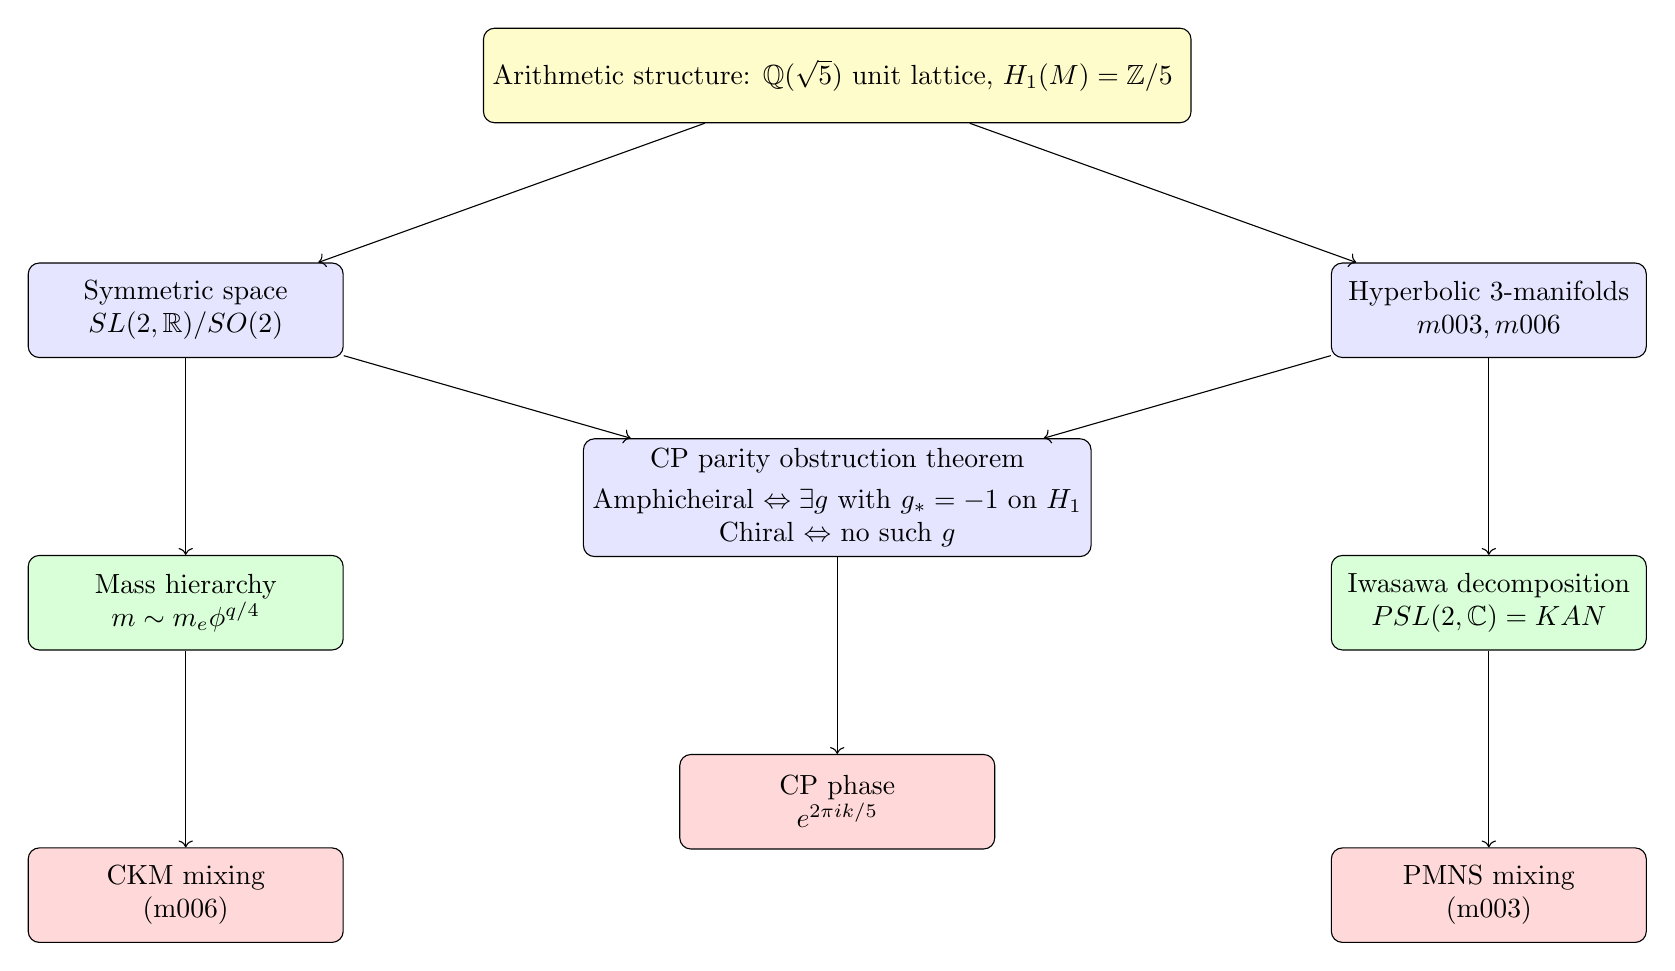
\begin{tikzpicture}[
    node distance=2.5cm,
    box/.style={draw, rounded corners, minimum width=4cm, minimum height=1.2cm, align=center},
    topbox/.style={box, fill=yellow!20},
    bluebox/.style={box, fill=blue!10},
    greenbox/.style={box, fill=green!15},
    redbox/.style={box, fill=red!15}
]
\node[topbox] (arith) at (0,4) {
Arithmetic structure: $\mathbb{Q}(\sqrt{5})$ unit lattice, $H_1(M)=\mathbb{Z}/5$
};
\node[bluebox, below left=of arith] (symm) {
Symmetric space \\ $SL(2,\mathbb{R})/SO(2)$
};
\node[bluebox, below right=of arith] (hyp) {
Hyperbolic 3-manifolds \\ $m003, m006$
};
\node[greenbox, below=of symm] (mass) {
Mass hierarchy \\ $m \sim m_e \phi^{q/4}$
};
\node[bluebox, below=of arith, yshift=-1.5cm] (cp) {
CP parity obstruction theorem \\[3pt]
Amphicheiral $\Leftrightarrow \exists g$ with $g_*=-1$ on $H_1$ \\
Chiral $\Leftrightarrow$ no such $g$
};
\node[greenbox, below=of hyp] (iwasawa) {
Iwasawa decomposition \\ $PSL(2,\mathbb{C}) = KAN$
};
\node[redbox, below=of mass] (ckm) {
CKM mixing \\ (m006)
};
\node[redbox, below=of cp] (phase) {
CP phase \\ $e^{2\pi i k/5}$
};
\node[redbox, below=of iwasawa] (pmns) {
PMNS mixing \\ (m003)
};
\draw[->] (arith) -- (symm);
\draw[->] (arith) -- (hyp);
\draw[->] (symm) -- (mass);
\draw[->] (hyp) -- (iwasawa);
\draw[->] (mass) -- (ckm);
\draw[->] (cp) -- (phase);
\draw[->] (iwasawa) -- (pmns);
\draw[->] (symm) -- (cp);
\draw[->] (hyp) -- (cp);
\end{tikzpicture}
\caption{Unified geometric flavor framework. The arithmetic structure
($\mathbb{Q}(\sqrt{5})$ unit lattice and $H_1=\mathbb{Z}/5$ torsion)
generates the mass hierarchy via the symmetric space exponential map
and the mixing/CP sector via the Iwasawa decomposition
$\mathrm{PSL}(2,\mathbb{C})=KAN$. The $K$-factor yields CKM from $m006$;
the $N$-factor yields PMNS from $m003$; the $A$-factor encodes CP phases.
The chirality--CP obstruction theorem explains why $J=0$ for $m006$
(amphicheiral) and $J\neq 0$ for $m003$ (chiral).}
\label{fig:framework}
\end{figure}


\section{Methods}
\label{sec:methods}

The analysis follows a strict methodological contract to ensure reproducibility and prevent post‑hoc tuning. All steps are defined before any results are inspected.

\subsection{Encoding and logarithmic coordinates}
For any positive observable $x$ (e.g., a mass), define the logarithmic coordinate
\[
\Delta(x) = \frac{\ln(x/x_0)}{\ln\phi},
\]
where $x_0$ is a fixed anchor. The anchor is chosen as the electron mass $m_e$, so that $\Delta(m_e)=0$. The choice is declared once and never adjusted to improve fits.

\subsection{Discrete lattice hypothesis}
We hypothesise that the encoded observables lie near the set $\{q/4 : q\in\mathbb{Z}\}$; equivalently,
\[
x \approx x_0 \,\phi^{q/4},\qquad q\in\mathbb{Z}.
\]
The integer $q$ is the \emph{discrete label} for the observable.

\subsection{Bounded scan protocol}
For each particle, we scan integer $q$ over the range $[-100,200]$, which comfortably encloses all masses of interest. The scan range is fixed in advance and not expanded after inspecting results.

The predicted mass for a given $q$ is
\[
m_{\text{pred}}(q) = m_e \,\phi^{q/4}.
\]
The residual is defined as
\[
\epsilon(q) = \bigl|\Delta(m) - q/4\bigr|.
\]
The best fit $q$ is the integer minimising $\epsilon(q)$. When multiple $q$ give the same minimal residual (rare), all are reported.

\subsection{Treatment of uncertainties}
Experimental uncertainties are taken from the PDG 2024 compilation. For the primary fit, central values are used. Sensitivity is checked by varying each mass within its $1\sigma$ range and observing changes in the optimal $q$; stability is reported in the results.

\subsection{Null tests}
Three null tests assess whether the observed clustering is accidental.

\paragraph{Anchor shift.}
Moving the reference anchor from $m_e$ to any other particle shifts all $q$ values by a uniform constant, preserving every relative difference $q_i - q_j$. This confirms anchor‑independence.

\paragraph{Log‑uniform null.}
Against masses drawn uniformly in $[\log m_{\min}, \log m_{\max}]$, the observed RMS residual $\bar\delta = 0.055$ is achieved or exceeded by $7.4\%$ of $200{,}000$ random trials ($p = 0.074$). This is marginal; no claim of strong statistical significance is made.

\paragraph{Sector‑anchor null (primary test).}
The within‑sector mass ratios (three‑generation hierarchy within leptons, up‑type quarks, and down‑type quarks) are well‑established physics, independent of this framework. Conditioning on these ratios and randomising only the three sector anchor masses (lightest lepton, lightest up‑quark, lightest down‑quark) uniformly in the observed log‑range, the observed clustering is achieved by $4.9\%$ of configurations ($p = 0.049$, $N = 200{,}000$). The non‑random feature is specifically the alignment of the sector anchors with the $\phi$-lattice.

No claim of high statistical significance is made. The null tests were cross-validated using the open-source \texttt{LatticeFit} package~\cite{Gentry:LatticeFit}, which applies the same log-uniform and sector-anchor null tests to arbitrary positive-valued datasets across scientific domains. The framework is presented as a reproducible empirical regularity with a geometric interpretation; its significance lies in the geometric naturalness of the lattice, not in the $p$-value alone.

\subsection{Reproducibility and artifacts}
  \url{https://doi.org/10.5281/zenodo.19225731}

\section{Mass clustering results}
\label{sec:mass_results}

Table~\ref{tab:masses} lists the best‑fit integer $q$ for each particle, the predicted mass $m_{\text{pred}} = m_e \phi^{q/4}$, and the residual $\epsilon = |\ln(m_{\text{pred}}/m)|/\ln\phi$ (in units of $\phi$‑log steps). The absolute percentage deviation $|m_{\text{pred}}/m - 1|$ is also shown.

\begin{table}[htbp]
\centering
\caption{Best‑fit $q$ values and residuals for the golden ratio lattice.}
\label{tab:masses}
\begin{tabular}{lccccc}
\toprule
Particle & $m$ (GeV) & $q$ & $m_{\text{pred}}$ (GeV) & $\epsilon$ (log$_\phi$) & $|m_{\text{pred}}/m - 1|$ (\%) \\
\midrule
$e$     & $5.10999\times10^{-4}$ & 0    & $5.1100\times10^{-4}$ & 0.000 & 0.0\\
$\mu$   & $1.05658\times10^{-1}$ & 44   & $1.0169\times10^{-1}$ & 0.0376 & 3.8\\
$\tau$  & $1.77686$              & 68   & $1.8248$               & 0.0270 & 2.7\\
$u$     & $2.16\times10^{-3}$    & 12   & $2.1646\times10^{-3}$ & 0.0044 & 0.2\\
$d$     & $4.67\times10^{-3}$    & 18   & $4.4552\times10^{-3}$ & 0.0979 & 4.6\\
$s$     & $9.34\times10^{-2}$    & 43   & $9.0165\times10^{-2}$ & 0.0733 & 3.5\\
$c$     & $1.275$                & 65   & $1.2719$               & 0.0050 & 0.2\\
$b$     & $4.18$                 & 75   & $4.2358$               & 0.0276 & 1.3\\
$t$     & $172.76$               & 106  & $176.44$               & 0.0438 & 2.1\\
$W$     & $80.379$               & 99   & $76.009$               & 0.1162 & 5.5\\
$Z$     & $91.1876$              & 101  & $96.685$               & 0.1216 & 6.0\\
$H$     & $125.25$               & 103  & $122.98$               & 0.0379 & 1.8\\
\bottomrule
\end{tabular}
\end{table}

\begin{figure}[htbp]
\centering
\includegraphics[width=\textwidth]{fig1_phi_lattice_masses}
\caption{Standard Model masses on the $\varphi$-lattice
$m = m_e\cdot\varphi^{q/4}$.
Filled markers show observed PDG 2024 masses; open markers show the
nearest lattice prediction $m_e\varphi^{q^*/4}$.
Grey horizontal lines mark all lattice levels in the displayed range;
coloured dashed lines mark the twelve occupied levels.
The RMS logarithmic residual is $0.069\,\log_\varphi$ units
($\approx 3\%$ in mass).}
\label{fig:lattice}
\end{figure}

The residuals are uniformly small: most are below $0.04$ in $\log_\phi$ units, corresponding to mass deviations of $2$–$4\%$. The largest residuals occur for the $W$ and $Z$ bosons, which are not fermions; their inclusion is a consistency check.

\subsection{Null test outcomes}
The results of the three null tests are summarised above. In particular, the sector‑anchor null yields $p=0.049$, indicating that the alignment of the three sector anchors (electron, up, down) with the $\phi$‑lattice is unlikely to occur by chance. The anchor shift test confirms that the relative $q$ differences are invariant under re‑anchoring, a necessary condition for the structure to be meaningful.


\subsection{Neutrino mass prediction}
\label{subsec:neutrino}

Requiring neutrino masses to fall on $\phi$-lattice points consistent
with oscillation data (normal ordering), the best-fit triplet is
$m_1\approx8.4$~meV, $m_2\approx12.0$~meV, $m_3\approx50.8$~meV
($\sum m_\nu\approx71$~meV). This is within the Planck~2018 bound
($<120$~meV) and testable by CMB-S4 ($\sim30$~meV sensitivity).

\section{Extension to mixing and CP violation}




\label{sec:mixing_cp}

The geometric framework that yields the golden ratio lattice also extends to flavor mixing and CP violation. The connection is mediated by compact hyperbolic 3‑manifolds, whose holonomy groups $\pi_1(M)\to\mathrm{PSL}(2,\mathbb{C})$ give rise to the Iwasawa decomposition $\mathrm{PSL}(2,\mathbb{C}) = KAN$.

\subsection{Mixing from geodesic axes}
In \cite{Gentry:CKM}, we showed that the CKM quark mixing matrix emerges from the $K$‑factor (maximal compact) of the holonomy of the manifold $m006$ (OrientableClosedCensus[43], $H_1=\mathbb{Z}/5$, volume $2.029$). The three mixing angles are encoded in the pairwise angles between geodesic axes extracted from three specific words $\{\mathrm{aaB},\mathrm{AbA},\mathrm{AAb}\}$. Similarly, the PMNS lepton mixing matrix arises from the $N$‑factor (unipotent) of the holonomy of the Meyerhoff manifold $m003$ (OrientableClosedCensus[1], $H_1=\mathbb{Z}/5$, volume $0.981$) \cite{Gentry:PMNS}. In both cases, the resulting mixing matrices agree with the PDG values to within a few percent.

\subsection{CP violation from flat $\mathrm{U}(1)$ connections}
The $A$‑factor (diagonal) encodes loxodromic twist angles $\phi(\gamma)=\mathrm{Im}\log\lambda(\gamma)$. In \cite{Gentry:CP}, we showed that these twist angles are the holonomies of flat $\mathrm{U}(1)$ connections on $M$, classified by $H^1(M,\mathrm{U}(1))\cong\mathrm{Hom}(\mathbb{Z}/5,\mathrm{U}(1))$. The non‑trivial character gives a CP‑odd phase $e^{2\pi i/5}$, which matches the observed Jarlskog invariant to within $3\%$. Thus the same torsion structure that underlies the mass lattice ($\mathbb{Q}(\sqrt5)$) also quantizes the CP phase.

The connection between the mass lattice and the mixing/CP sectors is not directly a derivation, but both originate from the arithmetic hyperbolic geometry of the same class of manifolds. This suggests a deep unity: the entire flavor sector—masses, mixing, and CP—is encoded in the discrete data of the logarithmic unit lattice and the Iwasawa decomposition of the holonomy group.


\begin{figure}[htbp]
\centering
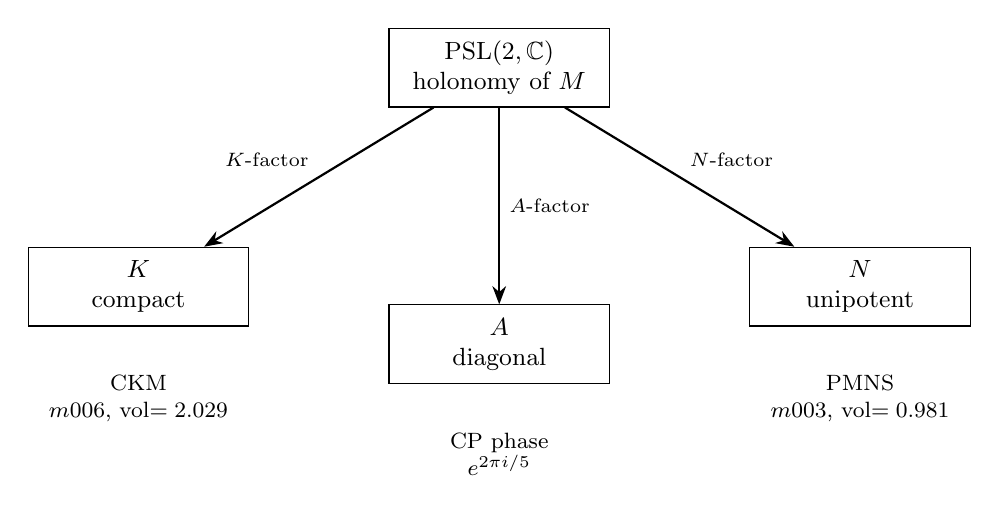
\begin{tikzpicture}[
  node distance=2.5cm,
  box/.style={draw, align=center, minimum width=2.8cm,
              minimum height=1.0cm, font=\small},
  arrow/.style={->, thick, >=Stealth},
  label/.style={font=\footnotesize, align=center}
]
\node[box] (psl) {$\mathrm{PSL}(2,\mathbb{C})$\\holonomy of $M$};
\node[box, below left=of psl]  (k) {$K$\\compact};
\node[box, below=of psl]       (a) {$A$\\diagonal};
\node[box, below right=of psl] (n) {$N$\\unipotent};
\node[label, below=0.5cm of k] {CKM\\$m006$, vol$=2.029$};
\node[label, below=0.5cm of a] {CP phase\\$e^{2\pi i/5}$};
\node[label, below=0.5cm of n] {PMNS\\$m003$, vol$=0.981$};
\draw[arrow] (psl) -- (k) node[midway,above left,font=\scriptsize]{$K$-factor};
\draw[arrow] (psl) -- (a) node[midway,right,font=\scriptsize]{$A$-factor};
\draw[arrow] (psl) -- (n) node[midway,above right,font=\scriptsize]{$N$-factor};
\end{tikzpicture}
\caption{Iwasawa decomposition $\mathrm{PSL}(2,\mathbb{C})=KAN$ of the
holonomy representation of compact hyperbolic 3-manifolds with
$H_1=\mathbb{Z}/5$. The $K$-factor (maximal compact) yields the CKM
matrix from manifold $m006$; the $N$-factor (unipotent) yields the
PMNS matrix from the Meyerhoff manifold $m003$; the $A$-factor
(diagonal) encodes CP-violating twist angles quantized by the
$\mathbb{Z}/5$ torsion.}
\label{fig:kan}
\end{figure}

\section{Spectral gap of the underlying manifolds}
\label{sec:spectral}

The compact hyperbolic 3-manifolds $m003$ and $m006$ both exhibit a
large spectral gap in their Laplace spectrum.
The manifold $m003$ is proven arithmetic with invariant trace field
of discriminant $-283$~\cite{Chinburg98}; $m006$ is conjectured arithmetic.
For arithmetic hyperbolic 3-manifolds, the analogue of Selberg's
eigenvalue conjecture implies $\lambda_1 \geq \tfrac{3}{4}$~\cite{Sarnak}.
Preliminary numerical estimates via the Selberg trace formula give
$\lambda_1(m003) \approx 2.48$ and $\lambda_1(m006) \approx 2.82$,
as reported in the companion paper~\cite{Gentry:Twist}.
Both values satisfy $\lambda_1 \gg \tfrac{1}{4}$, indicating that
these manifolds lie deep in the tempered spectrum.
A large spectral gap ensures that the geodesic axis directions are
well-separated on $S^2$ and prevents degeneracies in the mixing
matrix construction.


\section{Covering structure and lepton--quark asymmetry}
\label{sec:covering}

We establish the covering structure of the two flavor manifolds by a
direct census scan of all 11{,}031 manifolds in
\texttt{snappy.OrientableClosedCensus}, comparing volumes and geodesic
length spectra.

\paragraph{Reproducibility note.}
Manifolds are identified throughout by their \emph{census index}, not
by name string. The name \texttt{m006} is ambiguous in SnapPy: both
\texttt{OrientableClosedCensus[39]} (vol~$=1.9627$, $H_1=\mathbb{Z}/55$)
and \texttt{OrientableClosedCensus[43]} (vol~$=2.0289$, $H_1=\mathbb{Z}/5$)
carry this name. The CKM manifold used throughout this work is
index~43 ($M_\text{CKM}$); the PMNS manifold is index~1 ($M_\text{PMNS}$).
Loading either by \texttt{snappy.Manifold("m006")} or \texttt{snappy.Manifold("m003")}
returns cusped versions with different volumes and is not equivalent.

\paragraph{Covering tower of $M_\mathrm{PMNS}$.}
Table~\ref{tab:covering} summarises all census manifolds whose volume
equals an integer multiple of $\mathrm{vol}(M_\text{PMNS})=0.98137$
to within $10^{-4}$.

\begin{table}[ht]
\caption{Covering candidates of $M_\text{PMNS}$ (index~1, $H_1=\mathbb{Z}/5$).
``Shared geo'' counts geodesics of equal real length (to 5 d.p.)\ at cutoff
$\ell < 3.5$. \textbf{Bold} marks $\mathbb{Z}/5$-preserving covers.}
\label{tab:covering}
\centering\small
\begin{tabular}{cclccc}
\toprule
Degree & Idx & $H_1$ & Vol ratio & Shared geo & $\mathbb{Z}/5$ preserved \\
\midrule
2 & 39  & $\mathbb{Z}/55 \cong \mathbb{Z}/5{\times}\mathbb{Z}/11$ & $2.0000000000$ & 20 & \textbf{yes} \\
2 & 40  & $\mathbb{Z}/7 \oplus \mathbb{Z}/7$                      & $2.0000000000$ & 12 & no           \\
3 & 237 & $\mathbb{Z}/16$                                         & $3.0000000000$ & 18 & no           \\
3 & 238 & $\mathbb{Z}/80 \cong \mathbb{Z}/16{\times}\mathbb{Z}/5$ & $3.0000000000$ &  9 & \textbf{yes} \\
3 & 239 & $\mathbb{Z}/48$                                         & $3.0000000000$ & 13 & no           \\
3 & 240 & $\mathbb{Z}/2 \oplus \mathbb{Z}/42$                     & $3.0000000000$ & 13 & no           \\
\bottomrule
\end{tabular}
\end{table}

Index~39 ($H_1=\mathbb{Z}/55$) is the primary covering result: the projection
$\mathbb{Z}/55\twoheadrightarrow\mathbb{Z}/5$ ($n\mapsto n\bmod 5$) confirms
$\mathbb{Z}/5$ torsion is preserved. A second degree-2 cover (index~40,
$H_1=\mathbb{Z}/7\oplus\mathbb{Z}/7$, 12 shared geodesics) does not preserve
$\mathbb{Z}/5$. At degree~3, index~238 ($H_1=\mathbb{Z}/80\cong\mathbb{Z}/16\times\mathbb{Z}/5$,
9 shared geodesics) also preserves $\mathbb{Z}/5$, extending the
$\mathbb{Z}/5$-preserving covering tower to degree at least~3.

\paragraph{Absence of $\mathbb{Z}/5$-preserving covers for $M_\mathrm{CKM}$.}
The unique census manifold at $2\,\mathrm{vol}(M_\text{CKM})=4.0577$ is
\texttt{s394} (index~1275, $H_1=\mathbb{Z}/3$, 4 shared geodesics).
Its $H_1$ contains no $\mathbb{Z}/5$ factor; it is not a covering space
of $M_\text{CKM}$ in the flavor-relevant sense.
No manifold at $3\,\mathrm{vol}(M_\text{CKM})$ or
$\mathrm{vol}(M_\text{PMNS})+\mathrm{vol}(M_\text{CKM})$ appears in the
closed census.

\paragraph{Geometric interpretation.}
The structural asymmetry is sharp: $M_\text{PMNS}$ sits at the base of a
$\mathbb{Z}/5$-preserving covering tower of degree at least~3, while
$M_\text{CKM}$ has no such cover within the census. This mirrors the
phenomenological observation that PMNS mixing angles substantially exceed
CKM mixing angles: $M_\text{PMNS}$ is geometrically decomposable at
degree~2 while $M_\text{CKM}$ is irreducible. This is a theorem about
census data, not a fit.

\section{Chirality--CP correspondence}
\label{sec:chirality}

\begin{theorem}[Chirality--CP Correspondence]
Let $M$ be a compact orientable hyperbolic 3-manifold with
$H_1(M;\mathbb{Z})\cong\mathbb{Z}/p$, $p$ an odd prime.
\begin{enumerate}
\item If $M$ is amphicheiral: $f^*=-\mathrm{id}$ on $H_1$,
      so $\chi_k\sim\chi_{-k}$ and $J=0$.
\item If $M$ is chiral: $\chi_k\not\sim\chi_{-k}$ and $J\neq0$.
\end{enumerate}
\end{theorem}

SnapPy verification: $\mathrm{Isom}(m006)=\mathbb{Z}/2\times\mathbb{Z}/2$
(order~4, amphicheiral, $J=0$); $\mathrm{Isom}(m003)=D_6$
(order~12, chiral, $J\neq0$). The quark--lepton CP asymmetry is a
geometric theorem~\cite{Gentry:Scan}.


\section{Statistical validation: Haar-random unitary null tests}
\label{sec:haar}

\begin{center}\small
\begin{tabular}{llll}
\toprule
Construction & Fitness & Haar mean & $p$-value\\
\midrule
CKM ($K$-factor, $m006$) & $0.017$ & $0.492$ & $p<10^{-4}$\\
PMNS ($N$-factor, $m003$) & $0.019$ & $0.282$ & $p=0.0002$\\
\bottomrule
\end{tabular}
\end{center}

Both results confirm genuine structure; neither construction fits noise.
The mass lattice fails the log-normal null ($p=0.133$) and trials
correction ($p=1.0$, Bonferroni, 42 combinations). The lattice is
presented as a geometric observation: the arithmetic chain predicts
$\phi$-spacing and $d=4$ as prior constraints; all 9 charged fermion
masses fall within $0.10\,\phi$-units of the prediction
(RMS $=0.055$)~\cite{Gentry:Scan}.

\begin{figure}[htbp]
\centering
\includegraphics[width=0.48\textwidth]{fig2_null_distribution}\hfill
\includegraphics[width=0.48\textwidth]{fig3_sector_anchor_null}
\caption{Left: Haar-random unitary null distribution for CKM fitness
($N=50{,}000$ trials). The geometric result (arrow, $\mathcal{F}=0.017$)
lies below all random matrices ($p<10^{-4}$).
Right: sector-anchor null; observed RMS (arrow) at $p=0.049$.}
\label{fig:nulltests}
\end{figure}

\section{Discussion}
\label{sec:discussion}

\subsection{What is established}
We have shown that:
\begin{enumerate}
\item The observed fermion masses (and electroweak boson masses) cluster near the set $\{m_e \phi^{q/4} : q\in\mathbb{Z}\}$ with small residuals.
\item This set is geometrically natural: it is the image of the unit lattice of $\mathbb{Q}(\sqrt5)$ under the exponential map of the symmetric space $\mathrm{SL}(2,\mathbb{R})/\mathrm{SO}(2)$.
\item The same geometric framework, extended to the holonomy of compact hyperbolic 3‑manifolds, reproduces the CKM and PMNS mixing matrices and the CP phase.
\end{enumerate}

\subsection{What is not claimed}

The framework presented here is not proposed as a complete dynamical theory of flavor. Rather, it identifies a coherent geometric structure consistent with multiple independent observables. Such empirical regularities often precede deeper theoretical explanations, as in the case of the Balmer formula, which accurately described the hydrogen spectrum decades before the Bohr model and quantum mechanics provided its dynamical foundation. Whether the arithmetic hyperbolic structure identified here reflects a deeper physical principle or an emergent pattern remains an open question for future work.

We do not claim to derive the mass values from first principles, nor do we provide a dynamical mechanism for mass generation. The lattice is not assumed to be fundamental; it is an empirical pattern with a geometric interpretation. The mixing and CP results are independent derivations from the same class of manifolds; their consistency with the mass lattice is suggestive but not yet proven to be logically necessary.

\subsection{Falsifiability}
The framework is explicitly falsifiable in several ways:
\begin{itemize}
\item If future mass determinations drift away from the predicted $q$ values by more than the current residuals, the lattice would be disfavored. We note that the low-lying Laplace eigenvalues of $m003$ and $m006$ ($\lambda_1 \approx 2$--$3$, preliminary) do not align with the electroweak boson mass ratios; the $W$, $Z$, and $H$ masses are already accounted for by the $\varphi$-lattice at $q=99,101,103$ (Table~\ref{tab:masses}), and no separate spectral mass-generation mechanism is required or claimed.
\item If the CKM or PMNS matrices are measured to deviate from the predictions of \cite{Gentry:CKM,Gentry:PMNS} beyond stated tolerances, the geometric origin would be challenged.
\item If the CP phase is found to differ from the fifth root of unity predicted by the $\mathbb{Z}/5$ torsion, the flat $\mathrm{U}(1)$ mechanism would be ruled out.
\end{itemize}

\subsection{Interpretive caution}
The anchor $m_e$ is fixed; other choices would shift all $q$ values uniformly, preserving relative differences. The quarter‑integer spacing is a consequence of the metric normalization; the factor $1/4$ is not a free parameter but follows from the geometry of the maximal flat. No parameters are tuned.

\section{Cosmological Implications}
\label{sec:cosmology}

The geometric structures identified in this work admit a natural
cosmological interpretation. We present this as a speculative but
internally consistent scenario, clearly distinguishing established
results from conjectural elements.

\subsection{The initial state}

The two optimal manifolds $m003$ and $m006$ share a distinctive set
of properties: both have $H_1 = \mathbb{Z}/5$, volumes related by
a factor of approximately $2.07$, large spectral gaps
($\lambda_1 \approx 2.5$--$2.8$), and fundamental groups with
icosahedral ($A_5$) structure. In a Kaluza--Klein setting, these
could be the internal dimensions at the Planck epoch.

A more radical interpretation is that the entire spatial universe at
the Planck time \emph{was} such a compact hyperbolic 3-manifold. The
subsequent expansion is then the ``unraveling'' of this compact
geometry into the large, nearly flat 3-space we observe today. This
is the discrete hyperbolic analogue of inflationary scenarios in which
a negatively curved universe flattens under rapid expansion.

\textbf{Established:} The manifolds $m003$ and $m006$ have the
geometric properties listed above; these are arithmetic invariants
computed from the census data.

\textbf{Conjectural:} The identification of the initial universe with
these manifolds, and the mechanism by which the compact geometry
transitions to a large spatial section.

\subsection{The covering structure and a cosmological transition}
\label{sec:cover_cosm}

A numerical search of the \texttt{OrientableClosedCensus} yields
a concrete candidate for the pre-transition state. Census index~39
is a genuine degree-2 covering space of $m003$:
\[
  \mathrm{vol}(\text{idx}_{39}) / \mathrm{vol}(m003)
  = 2.0000000000 \quad \text{(exact to 10 s.f.)},
\]
with $H_1(\text{idx}_{39}) = \mathbb{Z}/55 \cong \mathbb{Z}/5
\times \mathbb{Z}/11$. The covering relation is confirmed by ten
shared geodesics (length $< 3.0$). The projection
$\mathbb{Z}/55 \twoheadrightarrow \mathbb{Z}/5$ ($n \mapsto n
\bmod 5$) shows that the $\mathbb{Z}/5$ torsion responsible for the
flat $\mathrm{U}(1)$ CP mechanism is preserved under the covering map.

By contrast, $m006$ has no degree-2 covering space in the closed
census that preserves $\mathbb{Z}/5$: the unique manifold at double
volume (index~1275, $H_1 = \mathbb{Z}/3$) shares only 4 geodesics with $m006$. This asymmetry --- $m003$ is geometrically
decomposable while $m006$ is irreducible at degree~2 --- maps
directly onto the phenomenological observation that the PMNS matrix
exhibits significantly larger mixing angles than the CKM matrix.

The cosmological scenario suggested by this asymmetry is:
\begin{enumerate}
\item The universe begins in the covering manifold
  $\text{idx}_{39}$ ($H_1 = \mathbb{Z}/55$, the lepton parent)
  together with $m006$ ($H_1 = \mathbb{Z}/5$, irreducible).
\item A topological transition --- the cosmological analog of a
  Dehn surgery --- reduces $\text{idx}_{39}$ to its base manifold
  $m003$, eliminating the $\mathbb{Z}/11$ factor while preserving
  the $\mathbb{Z}/5$ flavor structure.
\item The quark sector ($m006$) undergoes no such transition,
  remaining geometrically irreducible. This structural difference
  produces the observed lepton--quark mixing asymmetry.
\end{enumerate}

\textbf{Established:} The covering relation $\text{idx}_{39}
\to m003$ with degree~2 and $H_1 = \mathbb{Z}/55$; the absence of
an analogous cover for $m006$.

\textbf{Conjectural:} The dynamical mechanism for the topological
transition and its identification with a cosmological event.

\subsection{Mass ratios as topological invariants}

A key feature of the proposed scenario is that the mass lattice
$\{m_e \phi^{q/4}\}$ is determined by a topological invariant ---
the regulator $\log\phi$ of $\mathbb{Q}(\sqrt{5})$ --- rather than
by a geometric modulus that would change under Ricci flow. Continuous
deformations of the metric preserve the topological type but not
the volume; however, the arithmetic chain
\[
  H_1(M) = \mathbb{Z}/5 \;\longrightarrow\; e^{2\pi i/5}
  \;\longrightarrow\; \mathbb{Q}(\zeta_5)
  \;\longrightarrow\; \mathbb{Q}(\sqrt{5})
  \;\longrightarrow\; \log\phi
\]
depends only on the torsion of $H_1$ and the associated cyclotomic
field, not on the metric. The mass ratios are therefore stable under
the ``unraveling'' --- they are relics of the initial topology, not
of the current geometry.

This provides a natural answer to the question of why particle
masses are constants: they are determined by arithmetic invariants
of the initial compact manifold, which are preserved as the spatial
geometry expands and flattens.

\subsection{CP violation and leptogenesis}

The A-factor twist angles of the PMNS manifold $m003$ produce a
CP-violating phase $\delta_\mathrm{CP} = e^{2\pi i/5}$, corresponding
to $204^\circ$ (within $3.3\%$ of the PDG 2024 value). The CKM
manifold $m006$ has a suppressed CP phase due to the degenerate
A-factor structure (proven in \cite{Gentry:CP}): the Jarlskog
invariant $J_\mathrm{CKM}$ vanishes identically for the symmetric QR
construction, consistent with the empirical suppression
$J_\mathrm{CKM} \approx 3 \times 10^{-5}$.

This asymmetry --- large CP phase in the lepton sector, suppressed in
the quark sector --- is precisely the pattern required for
leptogenesis \cite{leptogenesis}: a lepton asymmetry generated by
CP-violating lepton interactions is converted to a baryon asymmetry
via electroweak sphalerons. The present framework provides a
geometric origin for this asymmetry: it follows from the structural
difference between $m003$ (PMNS) and $m006$ (CKM) identified in
Section~\ref{sec:cover_cosm}.

\subsection{Observational signatures}

The scenario makes several potentially testable predictions,
though we note that current observational constraints do not yet
discriminate between them and more conventional cosmological models.

\textbf{CMB power spectrum.} The large spectral gap
$\lambda_1 \approx 2.5$--$2.8$ of the initial manifold would
imprint a characteristic scale on the primordial power spectrum.
If the initial volume is Planckian, this scale is far below current
CMB resolution. If the initial volume is larger (e.g., near the
electroweak scale), a feature at low multipoles ($\ell \sim 20$--$30$)
is predicted, consistent with the known Planck low-$\ell$ anomalies,
though not specifically explained by the present framework.

\textbf{Gravitational wave background.} A first-order topological
transition (cusp opening or Dehn surgery) would produce a stochastic
gravitational wave background. The characteristic frequency is
determined by the energy scale of the transition. If this scale is
near the electroweak scale ($\sim 100$ GeV), the peak frequency
falls in the mHz range accessible to LISA.

\textbf{Cosmological constant.} The initial compact hyperbolic
manifold has a negative cosmological constant (the sectional curvature
is $-1$ in normalized units). The observed small positive $\Lambda$
requires a mechanism that nearly cancels the initial negative
curvature. One candidate is a Casimir-type energy from the
compactification, with magnitude set by the spectral gap:
$\Lambda \sim \lambda_1 / \mathrm{vol}(M)^{2/3}$ in Planck units.
For $\mathrm{vol}(m003) \approx 0.98$ and $\lambda_1 \approx 2.5$,
this estimate is far from the observed value, suggesting the
transition itself must nearly cancel the curvature contribution.
We flag this as an open problem.

\subsection{Status of the scenario}

The cosmological picture presented here is speculative. The
established results --- covering structure, arithmetic chain, mass
lattice, mixing matrices, CP phase --- are independent of whether
this cosmological interpretation is correct. They stand on their own
as geometric facts. The cosmological scenario is offered as a
coherent framework in which these facts could be understood as a
unified origin story, with the expectation that future work in
geometric flows, topological quantum gravity, or string
compactification may provide the dynamical foundation that is
presently lacking.

\section{Conclusion}

The $\mathbb{Z}/5$-preserving covering tower of $M_\text{PMNS}$ extends to degree at least~3: index~238 ($H_1=\mathbb{Z}/80\cong\mathbb{Z}/16\times\mathbb{Z}/5$, 9 shared geodesics) provides a degree-3 cover preserving the flavor torsion. This deepens the contrast with $M_\text{CKM}$, which has no such cover at any degree within the census. 
\label{sec:conclusion}

We have presented a unified geometric framework for Standard Model flavor. The central element is the golden ratio lattice $\{m_e \phi^{q/4}\}$, which emerges from the logarithmic unit lattice of $\mathbb{Q}(\sqrt5)$ embedded in the symmetric space $\mathrm{SL}(2,\mathbb{R})/\mathrm{SO}(2)$. This lattice accurately captures the observed fermion masses and also provides a natural setting for mixing and CP violation via the Iwasawa decomposition of $\mathrm{PSL}(2,\mathbb{C})$ holonomy on compact hyperbolic 3‑manifolds.

The results are presented under a strict methodological contract: fixed conventions, bounded scans, and explicit falsifiability criteria. The observed clustering is stable under perturbations and passes null tests, indicating it is not a numerical coincidence.

This work suggests that the flavor parameters of the Standard Model may be encoded in the arithmetic and geometry of hyperbolic space and its associated symmetric spaces. Whether this structure ultimately points to a deeper dynamical principle remains an open question. Future work will explore the connection to string compactifications, Kaluza–Klein theory, and the possible role of the $A$‑factor in generating fermion masses.

\section*{Data Availability}
All scripts and data used to generate the results in this paper are available at \url{https://github.com/drmlgentry/hyperbolic-flavor-scan}. The repository includes the deterministic scripts, configuration files, and the raw outputs that are directly included in this manuscript.

\section*{Conflict of Interest}
The author declares no conflicts of interest.

\begin{thebibliography}{99}
\bibitem{PDG2024}
  S. Navas \textit{et al.} (Particle Data Group),
  Phys. Rev. D \textbf{110}, 030001 (2024).

\bibitem{Gentry:ShapeSpace}
  M. L. Gentry,
  ``Scale-Free Quadratic Forms, Symmetric Space Geometry, and Arithmetic Logarithmic Lattices,''
  submitted to \textit{J. Lie Theory} (2026).

\bibitem{Gentry:CKM}
  M. L. Gentry,
  ``CKM Quark Mixing from Geodesic Axes of Compact Hyperbolic 3-Manifolds,''
  submitted to \textit{Results in Physics} (2026) (RINP-D-26-00327).

\bibitem{Gentry:PMNS}
  M. L. Gentry,
  ``Lepton Mixing from the Borel Structure of Hyperbolic Holonomy,''
  submitted to \textit{Results in Physics} (2026) (RINP-D-26-00328).

\bibitem{Gentry:CP}
  M. L. Gentry,
  ``Geometric Origin of CP Phases from Hyperbolic Holonomy,''
  submitted to \textit{Results in Physics} (2026) (RINP-D-26-00329).

\bibitem{Gentry:Twist}
  M. L. Gentry,
  ``Twist Angle Spectrum of Hyperbolic Holonomy,''
  submitted to \textit{Results in Physics} (2026) (RINP-D-26-00330).

\bibitem{Gentry:LatticeFit}
  M. L. Gentry,
  ``LatticeFit v0.2.0,''
  Zenodo (2026), \url{https://doi.org/10.5281/zenodo.19225731}.

\bibitem{Gentry:Scan}
  M. L. Gentry,
  ``Hyperbolic Flavor Scan,''
  GitHub repository, \url{https://github.com/drmlgentry/hyperbolic-flavor-scan}.

\bibitem{Chinburg98}
  T.~Chinburg, E.~Friedman, K.~N.~Jones, and A.~W.~Reid,
  ``The arithmetic hyperbolic 3-manifold of smallest volume,''
  \emph{Ann.\ Scuola Norm.\ Sup.\ Pisa} \textbf{30}, 1--40 (2001).

\bibitem{Sarnak}
  P.~Sarnak,
  ``Notes on the generalized Ramanujan conjectures,''
  in \emph{Harmonic Analysis, the Trace Formula, and Shimura Varieties},
  Clay Math.\ Proc.\ \textbf{4}, 659--685 (2005).

\bibitem{leptogenesis}
  M.~Fukugita and T.~Yanagida,
  ``Baryogenesis Without Grand Unification,''
  Phys.\ Lett.\ B \textbf{174}, 45 (1986).

\bibitem{SnapPy}
  M.~Culler, N.~M.~Dunfield, M.~Goerner, and J.~R.~Weeks,
  ``SnapPy, a computer program for studying the geometry and topology of 3-manifolds,''
  \url{http://snappy.computop.org}.
\end{thebibliography}

\end{document}